\chapter{Linux development}

In the previous chapters we went through the evolution of eBPF throughout the years and we analyzed all the components of its ecosystem.
Now we are ready to jump into some coding and write our first eBPF program.

We are going to start to talk about the development process on Linux, since historically it was the first operating system where eBPF was introduced and there is a greater and more complete documentation.
In fact, on the internet there are various tutorials and guides on writing your first eBPF program: however, we are going to present just a couple of projects that in our opinion are the best for starting with eBPF because they set up as many things as possible for beginner users to let them dive straight into writing eBPF programs and not get frustrated with various initials setup tasks.
Moreover, at the beginning of the history of eBPF it was necessary to work a lot from the Linux terminal for verifying, loading into the kernel and tearing down an eBPF program: however, the projects that we are going to present also simplify this procedure as well.

\section{Creation of the work environment}

The first requirement that we have to be met is that Linux is installed on our machine.
For our entire project, we used a computer with Windows 11 installed: this will be the host environment for all research and development activities. 
The computer has a 64 bit operating system with a processor based on x64, a 16 GB RAM and a Solid-State Drive (SSD) with a capacity of 1TB as for storage.
Windows 11, with its user-friendly interface and vast software ecosystem, combined with the power given by the four cores of the Intel Core i7 processor, provided an efficient platform for general computing requirements.

However, since we will have to work on another operating system, we have to take advantage of virtualization to create an isolated environment alongside the Windows host.
For installing and developing programs with eBPF on Linux, a virtual machine running Ubuntu 22.04 was set up within \textit{VirtualBox} (the version of the Ubuntu operating system must be at least the 20.10 because this and the following versions are Linux distributions that come with kernel BTF already built in).

VirtualBox is a type 2 (or hosted) hypervisor suitable for individual use and small-scale virtualization scenarios.
It is a software application that runs on top of an existing operating system (called host OS) and provides the capability to create and manage virtual machines. 
Figure \ref{fig:type_2_hypervisor} shows a schematic representation of the architecture just described.
VirtualBox allows you to test, develop and run multiple guest operating systems within your host operating system simultaneously, providing a good level of isolation between the host and guest operating systems.
As a type 2 hypervisor, VirtualBox relies on the host operating system's kernel to manage hardware resources: it uses device drivers and services from the host OS to interact with the physical hardware, which can introduce some overhead and may affect performance compared to a type 1 hypervisor.

\begin{figure}[h]
	\centering
	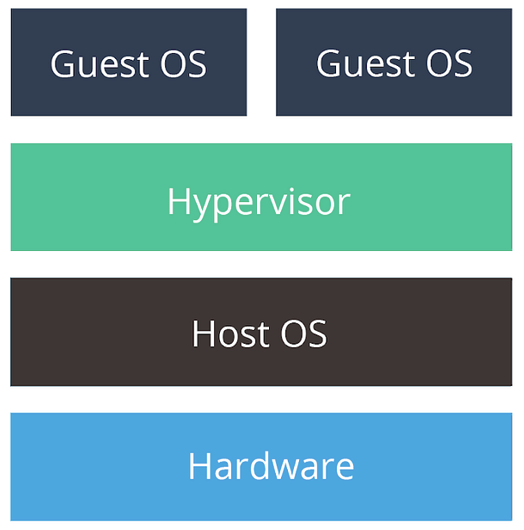
\includegraphics[width=0.7\linewidth]{images/Technologies/type_2_hypervisor.png}
	\caption{Type 2 (or hosted) hypervisor architecture \cite{HypervisorsArchitectures}.}
	\label{fig:type_2_hypervisor}
\end{figure}

Even though VirtalBox relies on the host OS for certain operations, which can lead to performance differences and potential resource conflicts, it was chosen over a type 1 hypervisor for its user-friendly virtualization solution.

The installation process involved creating a virtual disk, configuring memory and CPU allocation and selecting the Ubuntu 22.04 ISO file previously downloaded for installation \cite{UbuntuISOImage}. 
The virtual machine provided a native Linux platform for eBPF program development, compilation and testing.

\section{Bumblebee}

Every time anyone interfaces for the first time with something new, it is always nice to have anything ready with an explanation of what has been done in order to understand the new thing as quickly as possible.
This is exactly what happened when we came across \textit{BumbleBee} \cite{BumbleBeeWebsite} by \textit{solo.io}, a company known for its work in the field of cloud-native technologies, service mesh and API gateway solutions \cite{soloioWebsite}.

BumbleBee is an open-source project focused on simplifying the user experience around building eBPF tools \cite{BumbleBeeRepo}. 
It helps developers to build, run and distribute eBPF programs using Open Container Initiative (OCI) images, a standardized and portable way to package, distribute and run containerized applications across different container runtimes and platforms typically used in the DevOps and cloud-native ecosystem \cite{OCIRepo}.

By doing so, it allows the developer to focus on writing eBPF code, while taking care of the user space components.
We are going to see later that data is automatically exposed data as metrics or logs.

\subsection{Why BumbleBee}

In the previous chapters we understood that eBPF can run sandboxed programs in an operating system kernel to enhance the kernel capabilities with rapidly evolving network and security (to name a few) technologies.
Moreover, we went through its subsystem and the solution that was introduce to make eBPF programs portable across different kernel versions, i.e. BTF, a common type descriptor format.
However, nowadays packaging and sharing these binary programs is not very well specified. 
In fact, developers usually write the user-space code and the eBPF program, but they usually do have to figure out on their own how to distribute their application.

This is where BumbleBee comes into play: the idea is to use the same BTF typing to auto-generate all user-space code.
In fact, it is a tool that brings a Docker-like experience for automating critical steps in this process: its focus is on packaging, distribution and automatically generating user-space code for any eBPF program. 
By using a few and simple Command Line Interface (CLI, a text-based user interface
used to run programs, manage computer files and interact with the computer) commands it makes developing, running and distributing eBPF programs really simple.

BumbleBee is built using libbpf and allows the developer to focus on writing the eBPF code while automatically taking care of the user space components. 
Moreover, it detects and displays maps in the program that allow data sharing between user-space and kernel-space programs. 
Everything is done in complete autonomy by BumbleBee: the trick found in the use of special eBPF conventions and keywords, i.e. maps and functions, the two things that make up ebpf programs.

On the GitHub repository of the project there are a few examples of programs, but now we are going through all the process of developing a working eBPF program from scratch with the help of BumbleBee so we can more deeply understand how this projects works and how it makes the developer's life easier while interfacing for the first time with an eBPF program.

\subsection{Installation}

We presented earlier a way to create a Linux environment with the help of VirtualBox.
However, for non-Linux users, the BumbleBee project offers a Vagrant box \cite{BumblebeeVagrant} (with Docker, one of the main software for the portable deployment of application development environments) to help getting started with a Linux environment.
For the purpose of this thesis we are going to stick to the use of a virtual machine running the Linux operating system.

Being a Linux technology, eBPF should work in any Linux kernel.
However, the developers of BumbleBee suggest to run kernel 5.4 or newer.
Moreover,the Linux kernel of the machine must be built with \colorbox{backcolour}{\lstinline[style=highlight, language=bash]|CONFIG_DEBUG_INFO_BTF=y|} configuration because the projects relies on BPF CO-RE and BTF support.
A list of all the kernels that already support this configuration and a tutorial on how to build a custom kernel can be found on the libbpf GitHub repository \cite{BTFKernelConfig}.

Once the virtual machine is running, the first thing we need to do to get started with BumbleBee is to install the \colorbox{backcolour}{\lstinline[style=highlight, language=bash]|bee|} tool on our machine.
The easiest way to do so is to use the installation script provided by the project which does not even require to clone the repository on the machine.
Therefore, we have to open a terminal on our machine and write the following commands:

\begin{lstlisting}[style=commandline, language=bash, caption={bee installation commands}]
	sudo apt install curl
	sudo apt install docker.io 
	sudo -s
	curl -sL https://run.solo.io/bee/install | sh 
	export PATH=$HOME/.bumblebee/bin:$PATH
\end{lstlisting}

The first two commands must be performed only the first time the virtual machine is turned on and are important because they install the \colorbox{backcolour}{\lstinline[style=highlight, language=bash]|curl|} command (to make some browser calls from command line) and the package \colorbox{backcolour}{\lstinline[style=highlight, language=bash]|docker.io|}.
Instead, from line 3 to 5 there are three commands that must be executed every time the virtual machine is started up.
In particular:

\begin{itemize}
	\item 
		Line 3 is the standard way to give the user elevated privileges (these will be needed to run the \colorbox{backcolour}{\lstinline[style=highlight, language=bash]|bee|} command);
	\item 
		Line 4 installs the CLI and, in particular, downloads the latest \colorbox{backcolour}{\lstinline[style=highlight, language=bash]|bee|} version which is currently the 0.0.14 (if, for any reason, somebody wants to install a specific version \colorbox{backcolour}{\lstinline[style=highlight, language=bash]|x|}, it has to be specified \colorbox{backcolour}{\lstinline[style=highlight, language=bash]|BUMBLEBEE_VERSION=v0.0.8 sh|} in the command instead of just \colorbox{backcolour}{\lstinline[style=highlight, language=bash]|sh|});
	\item 
		Line 5 adds the \colorbox{backcolour}{\lstinline[style=highlight, language=bash]|bee|} CLI to \textit{PATH} (an environment variable that instructs a Linux system in which directories to search for executables and enables the user to run a command without specifying a path).
\end{itemize}

\subsection{Write an eBPF program}

Now that we have set up all the things that we need, we are ready to create our eBPF program.
The first thing that we have to do is to open a terminal and give the user elevated privileges.
Then we have to run the interactive command to bootstrap a new eBPF program.

\begin{lstlisting}[style=commandline, language=bash, caption={bee init command}]
	bee init
\end{lstlisting}

It will start a process of creating a program through a series of questions about the eBPF program you plan to build and will auto-generate the code template..
If, for any reason, the process has to be interrupted, it is enough to press \colorbox{backcolour}{\lstinline[style=highlight, language=bash]|CTRL+C|} at any moment.

The first choice that has to be done is about the language with which the program will be developed:

\begin{lstlisting}[style=commandline, language=bash, caption={bee language selection}]
	? What language do you wish to use for the filter: 
	- C
\end{lstlisting}

Currently only C is supported, but the company has planned the support for Rust as well.
In fact, a libbpf library for building eBPF applications in Rust which is called \textit{Libbpf-rs} \cite{libbpfRustGithubRepo}.
We will not enter in the details of this library since we have not used it: it is enough to know that it wraps eBPF functionality Rust-idiomatic interfaces and provides \textit{libbpf-cargo} plugin to handle eBPF code compilation and skeleton generation.
This library makes the building of the user-space part of the eBPF application in Rust easier.
However, the eBPF program themselves must still be written in plain C.

Selected the language, the process asks the type of program that is wanted.
\colorbox{backcolour}{\lstinline[style=highlight, language=bash]|bee|} has currently two hook points for the program: network or file system.
However, since eBPF enables developers to hook a program into any kernel functionality, we can expect that more of them will be added in the future.

\begin{lstlisting}[style=commandline, language=bash, caption={bee type of program selection}]
	? What type of program to initialize: 
	- Network
	File system
\end{lstlisting}

Network programs will primarily target integration with various functions within the kernel networking stack, whereas file-system programs will interface with file operations, including \textit{open()} calls.

Then, the interface questions about the desired type of global map for the eBPF program that is being built.
Once again, eBPF has several types of map, but \colorbox{backcolour}{\lstinline[style=highlight, language=bash]|bee|} currently implements only two of them: \colorbox{backcolour}{\lstinline[style=highlight, language=bash]|Ringbuffer|} and \colorbox{backcolour}{\lstinline[style=highlight, language=bash]|HasMap|}.

\begin{lstlisting}[style=commandline, language=bash, caption={bee map type selection}]
	? What type of map should we initialize: 
	- RingBuffer
	HashMap
\end{lstlisting}

\colorbox{backcolour}{\lstinline[style=highlight, language=bash]|RingBuffer|} is a generic map type that works as a queue and is usually used for the storage of many arbitrary data types.
However, to allow \colorbox{backcolour}{\lstinline[style=highlight, language=bash]|bee|} to take care of all the user-space code, it has been imposed that only one type of data can be stored in a \colorbox{backcolour}{\lstinline[style=highlight, language=bash]|Ringbuffer|}: in fact we will see that a type is stored in the map definition, but this parameter is used by \colorbox{backcolour}{\lstinline[style=highlight, language=bash]|bee|} to correctly parse the data and it is not used in the kernel map definition. 
\colorbox{backcolour}{\lstinline[style=highlight, language=bash]|Hashmap|}, instead, works as a traditional map with both keys and values.
Another substantial difference between the two types of maps is that \colorbox{backcolour}{\lstinline[style=highlight, language=bash]|Ringbuffer|} handles the data only once, while the \colorbox{backcolour}{\lstinline[style=highlight, language=bash]|Hashmap|} keeps its data until it is removed manually.

The last decision that has to be done is about the output format.
This is what makes BumbleBee really interesting: normally, to develop an eBPF application, a developer has to write a user-space and a kernel-space program, but \colorbox{backcolour}{\lstinline[style=highlight, language=bash]|bee|} handles automatically the maps data and requires only to write kernel-space code.

\begin{lstlisting}[style=commandline, language=bash, caption={bee output format selection}]
	? What type of output would you like from your map: 
	- print
	counter
	gauge
\end{lstlisting}

\colorbox{backcolour}{\lstinline[style=highlight, language=bash]|print|} tells that the data in the maps will be displayed as text and \colorbox{backcolour}{\lstinline[style=highlight, language=bash]|print|} can be event based (if \colorbox{backcolour}{\lstinline[style=highlight, language=bash]|RingBuffer|} is used as map) or timer based (if \colorbox{backcolour}{\lstinline[style=highlight, language=bash]|HashMap|} is used).
On the other hand, \colorbox{backcolour}{\lstinline[style=highlight, language=bash]|counter|} and \colorbox{backcolour}{\lstinline[style=highlight, language=bash]|gauge|} are two types of metrics that are currently supported (as before, new ones could be introduced with the evolution of BumbleBee): the first one is pretty self-explanatory and is used to count the number of times an event occurs, qhile the second one is used to track numeric values that can change over time.

In the end the last thing to do is to give a name to the file.

\begin{lstlisting}[style=commandline, language=bash, caption={bee file location}]
	BPF Program File Location: file_name.c
\end{lstlisting}

Instead of \colorbox{backcolour}{\lstinline[style=highlight, language=bash]|file_name|} put the name of the file: it will be saved in the directory from which the commands were executed.

If everything was done as explained, the following message will appear on the terminal:

\begin{lstlisting}[style=commandline, language=bash, caption={bee successful program creation message}]
	Successfully wrote skeleton BPF program
\end{lstlisting}

Now we have created our eBPF program.
It must be specified that once the program has been created it is possible to modify it to add a specific functionality to the kernel: however, after the generation of the program, the file will have read-only permissions.
So, the first thing that has to be done is to give all permissions to the file using the \colorbox{backcolour}{\lstinline[style=highlight, language=bash]|chmod|} tool.

Once the eBPF program is created, the next step is to compile it.
To do so, once again we have to use the \colorbox{backcolour}{\lstinline[style=highlight, language=bash]|bee|} tool.

\begin{lstlisting}[style=commandline, language=bash, caption={bee built command}]
	bee build file_name.c name:v1
\end{lstlisting}

This command compiles the program and creates an OCI packaged eBPF image thanks to a \textit{docker} build container that simplifies the building of the code.
Then, the OCI image ca be shared to popular OCI compliant registries (Docker registry, GitHub Container Repository, or Google Container Repository, etc.), put in a workflow or deployed in a working environment.
Once an OCI image is downloaded from somewhere, it will be unpacked into an OCI Runtime filesystem bundle which will be run by an OCI Runtime, according to the Runtime Specification.

Once the process of compilation ends, the following messages will appear on the terminal: 

\begin{lstlisting}[style=commandline, language=bash, caption={bee successful OCI creation messages}]
	Successfully compiled "file_name.c" and wrote it to "file_name.o"
	Saved BPF OCI image to name:v1
\end{lstlisting}

Now, under the same directory, we will have the eBPF program and the corresponding object file generated by the process of compilation.
The OCI image, instead, will be saved somewhere in the machine.

We want to point out that the name of the eBPF program \colorbox{backcolour}{\lstinline[style=highlight, language=bash]|file_name|} and the one of the OCI image \colorbox{backcolour}{\lstinline[style=highlight, language=bash]|name|} do not have to be the same: however, if the two names correspond, it is easier to understand from which programs different images originated.
Another important thing to say is the fact that if a program is modified after it has been compiled, the program has to go through a second process of compilation using the same command show above.
However, if the changes to the file are not accepted by the compiler, the compilation gets interrupted and the OCI image of the program before the changes is deleted.

With the following command it is possible to look at all the OCI images stored locally that are ready to be run.

\begin{lstlisting}[style=commandline, language=bash, caption={bee list command}]
	bee list
\end{lstlisting}

Finally, we can run our program with a simple command.

\begin{lstlisting}[style=commandline, language=bash, caption={bee run command}]
	bee run name:v1
\end{lstlisting}

\subsection{Some examples}

Now that we understood how to create an eBPF program using BumbleBee, it is time to look at some code.
There are seven possible programs that can be created with the process described above:

\begin{itemize}
	\item 
		Six for the \colorbox{backcolour}{\lstinline[style=highlight, language=bash]|Network|} program type (three output formats for each of the two map types gives in total six possible combinations);
	\item 
		One for the \colorbox{backcolour}{\lstinline[style=highlight, language=bash]|File system|} program type because it will not ask to choose the map type and the output format.
\end{itemize}

We are going to show just one example of an eBPF program as it is created by the \colorbox{backcolour}{\lstinline[style=highlight, language=bash]|bee|} tool and use it to discuss the various selection options.
The program that we are going to present  is created after doing the following choices:

\begin{lstlisting}[style=commandline, language=bash, caption={bee choices for first program}]
	INFO  Selected Language: C
	INFO  Selected Program Type: Network
	INFO  Selected Map Type: RingBuffer
	INFO  Selected Output Type: print
	INFO  Selected Output Type: BPF Program File Location my_prog.c
\end{lstlisting}

This is what the program will look like:

\begin{lstlisting}[style=cstyle, language=C, caption={bee first program}]
	#include "vmlinux.h"
	#include "bpf/bpf_helpers.h"
	#include "bpf/bpf_core_read.h"
	#include "bpf/bpf_tracing.h"
	#include "solo_types.h"
	
	// 1. Change the license if necessary 
	char __license[] SEC("license") = "Dual MIT/GPL";
	
	struct event_t {
		// 2. Add ringbuf struct data here.
	} __attribute__((packed));
	
	// This is the definition for the global map which both our
	// bpf program and user space program can access.
	// More info and map types can be found here: https://www.man7.org/linux/man-pages/man2/bpf.2.html
	struct {
		__uint(max_entries, 1 << 24);
		__uint(type, BPF_MAP_TYPE_RINGBUF);
		__type(value, struct event_t);
	} events SEC(".maps.print");
	
	SEC("kprobe/tcp_v4_connect")
	int BPF_KPROBE(tcp_v4_connect, struct sock *sk)
	{
		// Init event pointer
		struct event_t *event;
		
		// Reserve a spot in the ringbuffer for our event
		event = bpf_ringbuf_reserve(&events, sizeof(struct event_t), 0);
		if (!event) {
			return 0;
		}
		
		// 3. set data for our event,
		// For example:
		// event->pid = bpf_get_current_pid_tgid();
		
		bpf_ringbuf_submit(event, 0);
		
		return 0;
	}
\end{lstlisting}

Even though this program can appear really simple, there are many things to look at.
First, we have to appreciate how our decisions have structured the code:

\begin{itemize}
	\item 
		\colorbox{backcolour}{\lstinline[style=cstyle, language=C]|event_t|} is an empty struct (for now);
	\item 
		\colorbox{backcolour}{\lstinline[style=cstyle, language=C]|events|} is our \colorbox{backcolour}{\lstinline[style=highlight, language=bash]|RingBuffer|} eBPF map;
	\item 
		\colorbox{backcolour}{\lstinline[style=cstyle, language=C]|".maps.print"|} tells that we have chosen the \colorbox{backcolour}{\lstinline[style=highlight, language=bash]|print|} output format;
	\item 
		\colorbox{backcolour}{\lstinline[style=cstyle, language=C]|SEC("kprobe/tcp_v4_connect")|} indicates the \colorbox{backcolour}{\lstinline[style=highlight, language=bash]|Network|} program type;
	\item 
		\colorbox{backcolour}{\lstinline[style=cstyle, language=C]|BPF_KPROBE|} is our eBPF program represented as a normal C function in a specially-named section that will be loaded into the kernel.
\end{itemize}

Second, we have to understand some things about a generic eBPF program:

\begin{itemize}
	\item 
		The first five lines are just includes for using eBPF technology (\colorbox{backcolour}{\lstinline[style=cstyle, language=C]|bpf_helpers.h|}, \colorbox{backcolour}{\lstinline[style=cstyle, language=C]|bpf_core_read.h|} and \colorbox{backcolour}{\lstinline[style=cstyle, language=C]|bpf_tracing.h|}), kernel symbols (\colorbox{backcolour}{\lstinline[style=cstyle, language=C]|vmlinux.h|}) and types that bee can automatically interpret and display (\colorbox{backcolour}{\lstinline[style=cstyle, language=C]|solo_types.h|});
	\item 
		\colorbox{backcolour}{\lstinline[style=cstyle, language=C]|SEC("...")|} is a macro defined in \colorbox{backcolour}{\lstinline[style=cstyle, language=C]|bpf_helpers.h|} that puts variables and functions into the specified sections;
	\item 
		\colorbox{backcolour}{\lstinline[style=cstyle, language=C]|__license|} is a variable that defines the license of our eBPF code which is mandatory and enforced by the kernel (some eBPF functionality is unavailable to non-GPL-compatible code);
	\item 
		The program is attached to \colorbox{backcolour}{\lstinline[style=cstyle, language=C]|tcp_v4_connect|} through a kprobe, which means that every time we do a browser call (by searching anything in the browser or through the \colorbox{backcolour}{\lstinline[style=cstyle, language=C]|curl|} command) the function is triggered;
	\item 
		The second parameter of the function is a pointer to the struct which contains the information of the packet received when the program triggers the hook point and it must be done in this way because the program can only access valid memory spaces. 
		The only way to do so is to define through pointers all the header areas of the package which we intend to access with the written code.
\end{itemize}

Last, we have to look at the tricks that \colorbox{backcolour}{\lstinline[style=highlight, language=bash]|bee|} uses to take care of the user-space code.
In fact, this program is not what we will have to write if we were not working with \colorbox{backcolour}{\lstinline[style=highlight, language=bash]|bee|}.
There are a couple of things that are only present in programs generated with this tool: \colorbox{backcolour}{\lstinline[style=cstyle, language=C]|__type|} attribute in the map and \colorbox{backcolour}{\lstinline[style=cstyle, language=C]|".maps.print"|}.
In fact, we already said that \colorbox{backcolour}{\lstinline[style=highlight, language=bash]|RingBuffer|} is a map that can contain different types of data, but \colorbox{backcolour}{\lstinline[style=highlight, language=bash]|bee|} forces it to storage just one type of data.
Moreover, \colorbox{backcolour}{\lstinline[style=highlight, language=bash]|bee|} has to understand what type of output we want and to do so it adds \colorbox{backcolour}{\lstinline[style=cstyle, language=C]|.print|} inside the \colorbox{backcolour}{\lstinline[style=cstyle, language=C]|SEC|} macro of the eBPF map.
If we decided to use another output format, we will have \colorbox{backcolour}{\lstinline[style=highlight, language=bash]|counter|} or \colorbox{backcolour}{\lstinline[style=highlight, language=bash]|gauge|} in the place of \colorbox{backcolour}{\lstinline[style=highlight, language=bash]|print|}.

Despite all the efforts that we have made so far for creating and understanding this eBFP program, it does nothing.
In fact, if we compile and run the program we will see just a cool interface, but we will not display any information, as shown in Figure \ref{fig:bee_first_program_output}.

\begin{figure}[h]
	\centering
	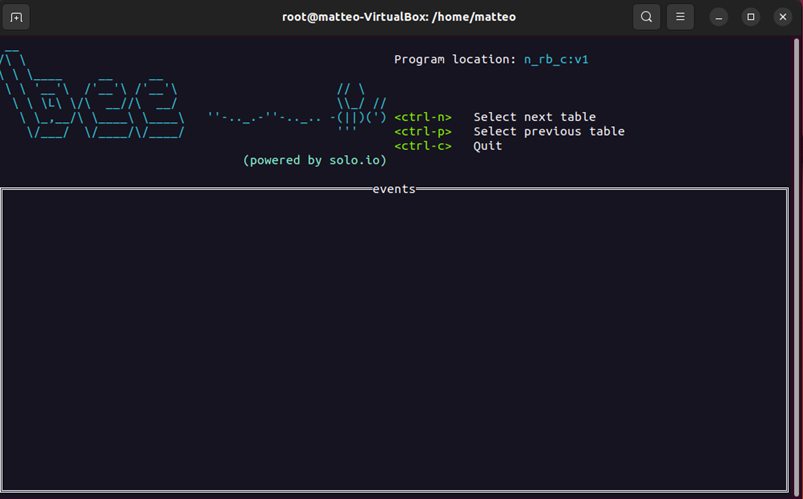
\includegraphics[width=0.7\linewidth]{images/LinuxDevelopment/n_rb_p_display.png}
	\caption{BumbleBee first program output.}
	\label{fig:bee_first_program_output}
\end{figure}

This is due to the fact that in out program the part where we have to set the data for the event (line 37) is commented.
To make things work we have to:

\begin{itemize}
	\item 
		Uncomment line 37 of our code;
	\item 
		Add \colorbox{backcolour}{\lstinline[style=cstyle, language=C]|u32 pid;|} inside the \colorbox{backcolour}{\lstinline[style=cstyle, language=C]|event_t|} struct;
\end{itemize}

\colorbox{backcolour}{\lstinline[style=cstyle, language=C]|u32|} is one of many variable types that is used by \colorbox{backcolour}{\lstinline[style=highlight, language=bash]|bee|} to take care of the user-space code in automatic: in practice, it is just a redefinition of the classical \colorbox{backcolour}{\lstinline[style=cstyle, language=C]|int|} type.

If we re-compile the program and re-run it, we should look at a terminal as displayed in Figure \ref{fig:bee_modified_first_program_output}.

\begin{figure}[h]
	\centering
	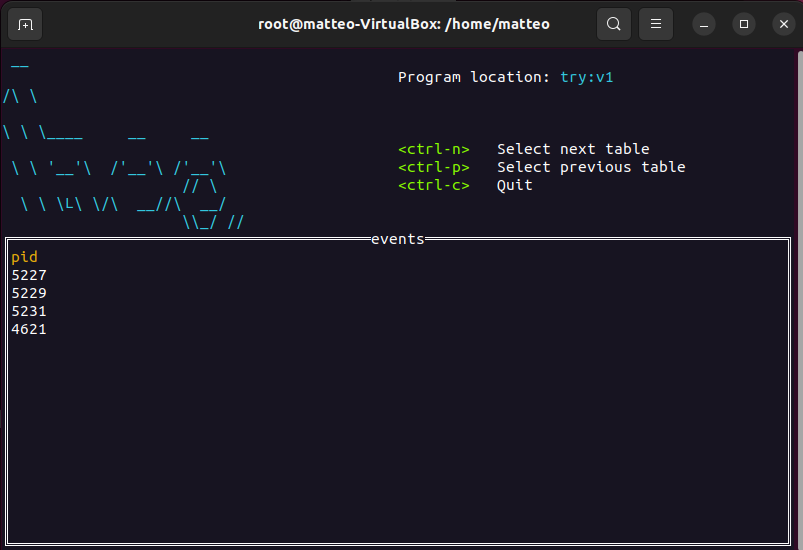
\includegraphics[width=0.7\linewidth]{images/LinuxDevelopment/n_rb_p_working_display.png}
	\caption{BumbleBee modified first program output.}
	\label{fig:bee_modified_first_program_output}
\end{figure}

Now we can see how the program really works: every time something happens in the kernel networking stack (e.g we search something on any browser), the eBPF program gets the ID (\textit{pid}) of the process and puts it in the \colorbox{backcolour}{\lstinline[style=highlight, language=bash]|RingBuffer|} with the use of just a few eBPF helpers.
Then, the ``magic'' behind \colorbox{backcolour}{\lstinline[style=highlight, language=bash]|bee|} shows it on the terminal.

With just a couple of changes in the script created by the \colorbox{backcolour}{\lstinline[style=highlight, language=bash]|bee|} tool we managed to develop a working eBPF program that shows us something interesting about the processes in the kernel networking stack.

Many things can be done with the following approach.
Now we are going to present a more complex example that contains more things of what we have presented.

\begin{lstlisting}[style=cstyle, language=C, caption={bee complex program}]
	#include "vmlinux.h"
	#include "bpf/bpf_helpers.h"
	#include "bpf/bpf_core_read.h"
	#include "bpf/bpf_tracing.h"
	#include "solo_types.h"
	
	// 1. Change the license if necessary 
	char __license[] SEC("license") = "Dual MIT/GPL";
	
	struct event_t {
		// 2. Add ringbuf struct data here.
		ipv4_addr daddr;
		u32 pid;
	} __attribute__((packed));
	
	struct dimensions_t {
		ipv4_addr daddr;
	} __attribute__((packed));
	
	struct {
		__uint(type, BPF_MAP_TYPE_HASH);
		__uint(max_entries, 8192);
		__type(key, struct dimensions_t);
		__type(value, u64);
	} connection_count SEC(".maps.counter");
	
	// This is the definition for the global map which both our
	// bpf program and user space program can access.
	// More info and map types can be found here: https://www.man7.org/linux/man-pages/man2/bpf.2.html
	struct {
		__uint(max_entries, 1 << 24);
		__uint(type, BPF_MAP_TYPE_RINGBUF);
		__type(value, struct event_t);
	} events SEC(".maps.print");
	
	
	SEC("kprobe/tcp_v4_connect")
	int BPF_KPROBE(tcp_v4_connect, struct sock *sk, struct sockaddr *uaddr) {
		struct event_t *event;
		struct dimensions_t hash_key = {};
		__u32 daddr;
		u64 counter;
		u64 *counterp;
		
		// read in the destination address
		struct sockaddr_in *usin = (struct sockaddr_in *)uaddr;
		daddr = BPF_CORE_READ(usin, sin_addr.s_addr);
		
		// Reserve a spot in the ringbuffer for our event
		event = bpf_ringbuf_reserve(&events, sizeof(struct event_t), 0);
		if (!event) {
			return 0;
		}
		// 3. set data for our event
		event->pid = bpf_get_current_pid_tgid();
		event->daddr = daddr;
		// submit the event (this makes it available for consumption)
		bpf_ringbuf_submit(event, 0);
		
		// increment the counter for this address
		hash_key.daddr = daddr;
		counterp = bpf_map_lookup_elem(&connection_count, &hash_key);
		if (counterp) {
			__sync_fetch_and_add(counterp, 1);
		} else {
			// we may miss N events, where N is number of CPUs. We may want to 
			// fix this for prod, by adding another lookup/update calls here.
			// we skipped these for brevity
			counter = 1;
			bpf_map_update_elem(&connection_count, &hash_key, &counter, BPF_NOEXIST);
		}
		
		return 0;
	}
\end{lstlisting}

The starting point of this program is the same of the previous one, but we have written a few more lines of code to develop a more advanced (but still simple) logic:

\begin{itemize}
	\item 
		There are two structs that are used for storing two different types of data in two different maps;
	\item 
		The program uses both a \colorbox{backcolour}{\lstinline[style=highlight, language=bash]|RingBuffer|} and an \colorbox{backcolour}{\lstinline[style=highlight, language=bash]|HashMap|} with two different output formats, respectively \colorbox{backcolour}{\lstinline[style=highlight, language=bash]|print|} and \colorbox{backcolour}{\lstinline[style=highlight, language=bash]|counter|};
\end{itemize}

The \colorbox{backcolour}{\lstinline[style=highlight, language=bash]|RingBuffer|} stores \colorbox{backcolour}{\lstinline[style=cstyle, language=C]|event_t|} data which contains the process ID and the destination address (of type \colorbox{backcolour}{\lstinline[style=cstyle, language=C]|ipv4_addr|}) of the network call.
The \colorbox{backcolour}{\lstinline[style=highlight, language=bash]|HashMap|}, instead, is a key-value store: the key consists of \colorbox{backcolour}{\lstinline[style=cstyle, language=C]|dimensions_t|} data (which is just the destination address) and the value is a classic \colorbox{backcolour}{\lstinline[style=cstyle, language=C]|long|} variable (redefined as \colorbox{backcolour}{\lstinline[style=cstyle, language=C]|u64|}).
The idea of the program is that get the id of the process that makes the browser call and its destination address and you store it in the \colorbox{backcolour}{\lstinline[style=highlight, language=bash]|RingBuffer|}.
Then, we increase the number of times that destination address has been searched.
To do so, we have to work with the \colorbox{backcolour}{\lstinline[style=highlight, language=bash]|HashMap|} and make use of a few more helpers to interact with a different eBPF map. 

\begin{itemize}
	\item 
		We check in the map if that destination address already exists;
	\item 
		If so, we increase the value associated to that address by 1;
	\item 
		If not, we put the new destination address as a new key in the map and its corresponding value is set to 1.
\end{itemize}

In Figure \ref{fig:bee_compelte_program_output} we can see the output that will appear on our terminal after we compile and run the program that we just showed and we make a few browser calls.

\begin{figure}[h]
	\centering
	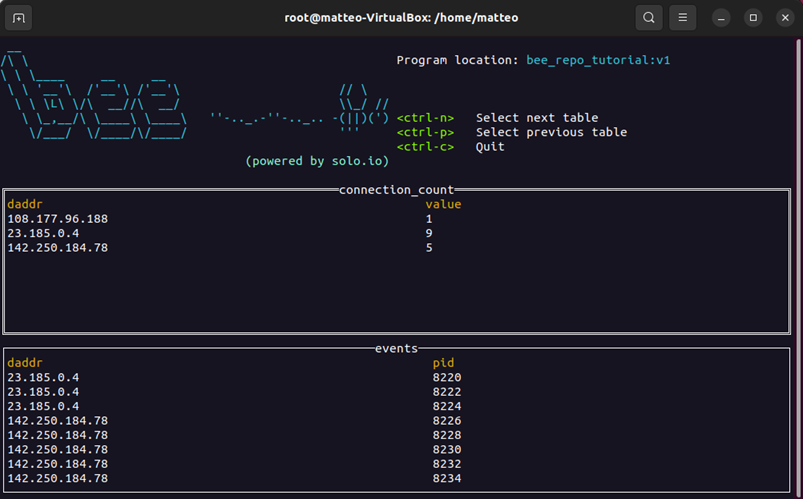
\includegraphics[width=0.7\linewidth]{images/LinuxDevelopment/bee_repo_tut_display.png}
	\caption{BumbleBee complete program output.}
	\label{fig:bee_compelte_program_output}
\end{figure}

Now that we can see the output, things get much more clear.
There are two sections delimited by two white rectangles: \textit{connection\_count} and \textit{events}, which correspond respectively to the \colorbox{backcolour}{\lstinline[style=highlight, language=bash]|HashMap|} and the \colorbox{backcolour}{\lstinline[style=highlight, language=bash]|RingBuffer|}.
In each box we can find the information contained in each map:

\begin{itemize}
	\item 
		In \textit{connection\_count} we find the destination address of the network call and the number of times this address has been reached;
	\item 
		In \textit{events} we fin the destination address and the id of the process that made the browser call.
\end{itemize}

This is just a quick sample of what can be written in a program generated with the \colorbox{backcolour}{\lstinline[style=highlight, language=bash]|bee|} tool.
Obviously the possibilities are much more than those shown, but we think that this is a good starting point to delve into the eBPF world.

\section{libbpf-bootstrap}

We have seen that BumbleBee greatly simplifies the development of an eBPF application since it takes care of many things: it generates all the code on which the eBPF program can be built and it manages the user-space part all by itself.
However, for the purpose of this thesis, we need to study the development of an eBPF program more thoroughly by writing from scratch both the kernel-side and the user-side code.

Although this may seem difficult, luckily for us it comes to our aid \textit{libbpf-bootstrap}, a project created, among other people, by Andrii Nakryiko and put on GitHub \cite{libbpfbootstrapGithubRepo}.
The idea behind this project is to provide an environment where as many things as possible are set up for beginner users to let them dive straight into writing eBPF programs in C without worrying about the initial setup.
In fact, at this point we might have understood that to give developers lots of power to extend the kernel functionalities without much kernel experience, eBPF requires the setup of a workflow through a series of steps that a new user has to unnecessarily know.
libbpf-bootstrap handles this task and provides a convenient workflow with the best eBPF user experience to date.

\subsection{Installation and overview}

Being a GitHub repository, to install this project on out Virtual Machine that runs Ubuntu 22.04 we have to just clone it locally with the following terminal command:

\begin{lstlisting}[style=commandline, language=bash, caption={libbpf-bootstrap clone command}]
	git clone --recurse-submodules https://github.com/libbpf/libbpf-bootstrap
\end{lstlisting}

By doing this, we also install the submodules that libbpf-bootstrap requires, such as  libbpf to exploit the BPF CO-RE concept and \textit{bpftool} to build skeleton files from the eBPF code.
More over, there is a simple \colorbox{backcolour}{\lstinline[style=highlight, language=bash]|Makefile|} that, although it can't be used directly, it's simple enough to just transfer the logic to whichever build system needs to be used.

The only thing that is missing on this repository is the compiler.
We already mentioned that to compile a C eBPF program we have to use Clang.
Even if Clang 10 should work fine for most eBPF features, the best thing that a user can do is to use the latest possible version: in fact, some features (some of the more recent and advanced CO-RE relocation built-ins) may require version 11 or 12.
Furthermore, the system should also have \colorbox{backcolour}{\lstinline[style=highlight, language=bash]|zlib|} and \colorbox{backcolour}{\lstinline[style=highlight, language=bash]|libelf|} packages installed because they are necessary for libbpf to compile and run programs properly.
To install all of these dependencies we just have to run the following prompt command:

\begin{lstlisting}[style=commandline, language=bash, caption={libbpf-bootstrap install dependencies command}]
	sudo apt install clang libelf1 libelf-dev zlib1g-dev
\end{lstlisting}

The last thing that we have to check is that since this projects relies on \textit{BTF CO-RE} and BTF kernel support, the  Linux kernel has to be built with \colorbox{backcolour}{\lstinline[style=highlight, language=bash]|CONFIG_DEBUG_INFO_BTF=y|} (as it was before for BumbleBee).

Finally, with just a couple of terminal commands, we are all set up to create and run our first eBPF program from scratch.
However, if anybody wants to take a further look inside some working programs, libbpf-bootstrap comes with a series of simple and documented examples both in C and Rust.
Moreover, having provided one of the major contributions to this project, Andrii Nakryiko published a post on his blog about the \colorbox{backcolour}{\lstinline[style=highlight, language=bash]|libbp-bootstrap|} environment where it talks about some simple examples in the repository and explains in detail how the \colorbox{backcolour}{\lstinline[style=highlight, language=bash]|Makefile|} works \cite{ANlibbpfbootstrap}.

\subsection{``Hello world!'' with eBPF}

Every time anyone has to deal with a new programming language or technology, the first program that is presented is and ``Hello world!''-like program.
To explain how we can write the kernel-side and the user-side of an eBPF program from scratch and make it work in the libbpf-bootstrap environment, we are going to do exactly what mentioned above.

The one thing that we have to keep in mind when working with libbpf-bootstrap is that both the programs must have the same name: the difference can be seen by the extensions of these files.
This is a very important naming convention since it helps the \textit{Makefile} to compile all the eBPF applications.
For the following example, we will call our program \colorbox{backcolour}{\lstinline[style=highlight, language=bash]|example_helloworld|}.

First, we show the eBPF C code that contain the logic which is going to be executed in the kernel context: this file has extension \colorbox{backcolour}{\lstinline[style=highlight, language=bash]|.bpf.c|} and has to be created under the \colorbox{backcolour}{\lstinline[style=highlight, language=bash]|libbpf-bootstrap/examples/c|} directory.
We also have to create the user-side program with extension \colorbox{backcolour}{\lstinline[style=highlight, language=bash]|.c|} because it will be required in the process of compilation.
However, we will keep this file empty (for now).

\begin{lstlisting}[style=cstyle, language=C, caption={``Hello world!'' kernel side program using libbpf-bootstrap}, title=example\_helloworld.bpf.c]
	#include "vmlinux.h"
	#include <linux/bpf.h>
	#include <bpf/bpf_helpers.h>
	
	char LICENSE[] SEC("license") = "Dual BSD/GPL";
	
	SEC("tracepoint/syscalls/sys_enter_execve")
	int bpf_prog(void *ctx) {
		char msg[] = "Hello, World!";
		bpf_printk("invoke bpf_prog: %s\n", msg);
		return 0;
	}
\end{lstlisting}

This program is really simple, but if we want to understand how to create a eBPF program from scratch there are a few things to look at:

\begin{itemize}
	\item 
		All the reported includes are a must for almost every eBPF program: we already	greatly discussed about \colorbox{backcolour}{\lstinline[style=cstyle, language=C]|vmlinux.h|}, but usually an application makes use of some basic eBPF-related types and constants necessary for using the kernel-side BPF APIs (included in \colorbox{backcolour}{\lstinline[style=cstyle, language=C]|linux/bpf.h|}) and macros, constants and eBPF helper definitions (included in \colorbox{backcolour}{\lstinline[style=cstyle, language=C]|bpf_helpers.h|} provided by libbpf);
	\item 
		\colorbox{backcolour}{\lstinline[style=cstyle, language=C]|SEC(...)|} and \colorbox{backcolour}{\lstinline[style=cstyle, language=C]|LICENSE|} are reported for the same reasons as we already discussed for the BumbleBee examples;
	\item 
		This time the code defines a tracepoint eBPF program which will be called every time an \colorbox{backcolour}{\lstinline[style=highlight, language=bash]|execve|} system call is invoked from any user-space application (in other words, every time we open a new application on our machine).
	\item 
		\colorbox{backcolour}{\lstinline[style=cstyle, language=C]|bpf_printk(...)|} is the eBPF equivalent to \colorbox{backcolour}{\lstinline[style=cstyle, language=C]|printf(...)|}. 
		The printed messages can be read from a special \colorbox{backcolour}{\lstinline[style=highlight, language=bash]|/sys/kernel/debug/tracing/trace_pipe|} file (we will see later how to display it).
\end{itemize}

The logic of the program is self-explanatory: every time an \colorbox{backcolour}{\lstinline[style=highlight, language=bash]|execve|} is invoked, the program prints the message \colorbox{backcolour}{\lstinline[style=highlight, language=bash]|invoke bpf_prog: Hello, World!|}.
We decided to just use this helper since it is the fastest and most convenient way for debugging a problem in an eBPF code.
In fact, eBPF does not have a debugger that does the conventional things (setting a breakpoint, inspecting variables and maps or single-stepping through the code) and to understand what is going on in out eBPF program we just have to rely on logging some information about it.
Due to its format, this helper is simple and easy to use, but it is computationally expensive, making it appropriate only for ad-hoc debugging and unsuitable to be used in production.
In reality, \colorbox{backcolour}{\lstinline[style=cstyle, language=C]|bpf_printk()|} is a macro defined by libbpf inside the \colorbox{backcolour}{\lstinline[style=cstyle, language=C]|bpf/bpf_helpers.h|} and internally calls the eBPF helper \colorbox{backcolour}{\lstinline[style=cstyle, language=C]|bpf_trace_printk()|}.
We are not going to talk about this anymore: whoever wants more details can visit the Andrii Nakryiko's blog and read the post about this topic \cite{ANbpfprintk}.

By just the few examples that we have covered, we could say that the trigger of our eBPF program is one of the most important things, if not the most important, because it reflects the hook point to which the program will attach: we could have different programs for different tracepoints or some other kernel events or define multiple programs with the same \colorbox{backcolour}{\lstinline[style=cstyle, language=C]|SEC(...)|} attribute.
Moreover, we could declare multiple eBPF programs inside the same eBPF C code and they will share all the global state which is useful when we try to make different programs collaborate.
Luckily, on the Linux kernel documentation there is a page with a complete explanation about program types and sections \cite{SecLinuxKernelDoc}.
Furthermore, libbpf exposes a detailed list of expected names on its GitHub repository \cite{SecListlibbpf}.

Once we have our kernel-side program, the next step that we have to do is to modify the \colorbox{backcolour}{\lstinline[style=highlight, language=bash]|Makefile|} under the same \colorbox{backcolour}{\lstinline[style=highlight, language=bash]|libbpf-bootstrap/examples/c|} directory by adding the name of our program (e.g. \colorbox{backcolour}{\lstinline[style=highlight, language=bash]|example_helloworld|}) after de \colorbox{backcolour}{\lstinline[style=highlight, language=bash]|APP|} variable.
We are not going to cover all the detail of this file: it is enough to know that it takes care the process of compilation of this program.

Now it is time to compile our program: to do so, we have to open a terminal with root privileges and once we go in the \colorbox{backcolour}{\lstinline[style=highlight, language=bash]|libbpf-bootstrap/build|} folder of our local copy of libbpf-bootstrap, we have to type the following commands:

\begin{lstlisting}[style=commandline, language=bash, caption={libbpf-bootstrap programs compilation commands}]
	cmake ../examples/c
	make
\end{lstlisting}

This is all it takes to compile our program.
By doing this, in the \colorbox{backcolour}{\lstinline[style=highlight, language=bash]|libbpf-bootstrap/build|} folder a few files will be generated.
In particular:

\begin{itemize}
	\item 
		After the first command, inside the \colorbox{backcolour}{\lstinline[style=highlight, language=bash]|CMakeFiles|} sub-folder, a sub-folder of extension \colorbox{backcolour}{\lstinline[style=highlight, language=bash]|.dir|} containing a series of files that will be used in the process of compilation will be created for each application specified in the \colorbox{backcolour}{\lstinline[style=highlight, language=bash]|Makefile|} (in our case, we will find the \colorbox{backcolour}{\lstinline[style=highlight, language=bash]|example_helloworld.dir|} sub-folder);
	\item 
		After the second command, the skeleton header, the object file and the executable file of the program will be generated.
\end{itemize}

If we want to speed up the process of compilation, we can specify the name of the only application that we want to compile in the second command (in our case, this would be \colorbox{backcolour}{\lstinline[style=highlight, language=bash]|make example_helloworld|}).

Now that we have generated it, it is time to analyze the skeleton header.
This is a big file (388 lines in the case of our program) due to the fact that it includes the bytecode representation of our program, so we are going to show only the most important parts and omit the implementations of various methods.

\begin{lstlisting}[style=cstyle, language=C, caption={``Hello world!'' skeleton file using libbpf-bootstrap}, title=example\_helloworld.skel.h]
	/* SPDX-License-Identifier: (LGPL-2.1 OR BSD-2-Clause) */
	
	/* THIS FILE IS AUTOGENERATED BY BPFTOOL! */
	#ifndef __EXAMPLE_HELLOWORLD_BPF_SKEL_H__
	#define __EXAMPLE_HELLOWORLD_BPF_SKEL_H__
	
	#include <errno.h>
	#include <stdlib.h>
	#include <bpf/libbpf.h>
	
	struct example_helloworld_bpf {
		struct bpf_object_skeleton *skeleton;
		struct bpf_object *obj;
		struct {
			struct bpf_map *rodata_str1_1;
			struct bpf_map *rodata;
		} maps;
		struct {
			struct bpf_program *bpf_prog;
		} progs;
		struct {
			struct bpf_link *bpf_prog;
		} links;
		
		#ifdef __cplusplus
		static inline struct example_helloworld_bpf *open(const struct bpf_object_open_opts *opts = nullptr);
		static inline struct example_helloworld_bpf *open_and_load();
		static inline int load(struct example_helloworld_bpf *skel);
		static inline int attach(struct example_helloworld_bpf *skel);
		static inline void detach(struct example_helloworld_bpf *skel);
		static inline void destroy(struct example_helloworld_bpf *skel);
		static inline const void *elf_bytes(size_t *sz);
		#endif /* __cplusplus */
	};
	
	...
	
	#endif /* __EXAMPLE_HELLOWORLD_BPF_SKEL_H__ */
\end{lstlisting}

The most important thing about this file is the \colorbox{backcolour}{\lstinline[style=highlight, language=bash]|example_helloworld_bpf|} struct: it contains a series of fields and methods that we can be directly used and accessed in our user-space program.
In particular:

\begin{itemize}
	\item 
		The struct \colorbox{backcolour}{\lstinline[style=cstyle, language=C]|bpf_object *obj|} can be passed to libbpf API functions;
	\item 
		\colorbox{backcolour}{\lstinline[style=cstyle, language=C]|maps|} contains all the maps defined in the kernel-side code with \colorbox{backcolour}{\lstinline[style=cstyle, language=C]|SEC(".maps")|}, plus the standard \colorbox{backcolour}{\lstinline[style=cstyle, language=C]|rodata|} pointer (we can have more than just one map in a single kernel-side code);
	\item 
		\colorbox{backcolour}{\lstinline[style=cstyle, language=C]|progs|} and \colorbox{backcolour}{\lstinline[style=cstyle, language=C]|links|} contain the pointers to the eBPF programs defined in our code with \colorbox{backcolour}{\lstinline[style=cstyle, language=C]|SEC("tracepoint")|} which, in our case, is just \colorbox{backcolour}{\lstinline[style=cstyle, language=C]|bpf_prog|} (we can have more than just one program in a single kernel-side code);
	\item 
		\colorbox{backcolour}{\lstinline[style=cstyle, language=C]|*bss|}, \colorbox{backcolour}{\lstinline[style=cstyle, language=C]|*data|} and \colorbox{backcolour}{\lstinline[style=cstyle, language=C]|*rodata|} are optional structs that can be used to allow direct access to eBPF global variables (they are not present in our skeleton file because we do no declare them).
		These sections are created if we define in the kernel-side program, respectively, zero-initialized and mutable or non-zero-initialized and mutable or read-only variables;
	\item 
		The methods \colorbox{backcolour}{\lstinline[style=cstyle, language=C]|open_and_load|}, \colorbox{backcolour}{\lstinline[style=cstyle, language=C]|open|}, \colorbox{backcolour}{\lstinline[style=cstyle, language=C]|load|}, \colorbox{backcolour}{\lstinline[style=cstyle, language=C]|attach|}, \colorbox{backcolour}{\lstinline[style=cstyle, language=C]|detach|} and \colorbox{backcolour}{\lstinline[style=cstyle, language=C]|destroy|} will be used to perform the now known standard operations on an eBPF program;
	\item 
		The method \colorbox{backcolour}{\lstinline[style=cstyle, language=C]|elf_bytes|} contains the bytecode representation of the kernel-side program.
\end{itemize}

Last, we present the user-space C code (remember that we left it empty in the \colorbox{backcolour}{\lstinline[style=highlight, language=bash]|libbpf-boostrap/examples/c|} folder), which loads eBPF code and interacts with it throughout the lifetime of the application.
Just for completeness, it is possible to define a \colorbox{backcolour}{\lstinline[style=highlight, language=bash]|.h|} header file with the common type definitions and is shared by both eBPF and user-space code of the application.
To keep things as simple as possible, we did not do that.

\begin{lstlisting}[style=cstyle, language=C, caption={``Hello world!'' user side program using libbpf-bootstrap}, title=example\_helloworld.c]
	#include <stdio.h>
	#include <unistd.h>
	#include <sys/resource.h>
	#include <bpf/libbpf.h>
	#include "example_helloworld.skel.h"
	
	static int libbpf_print_fn(enum libbpf_print_level level, const char *format, va_list args)
	{
		return vfprintf(stderr, format, args);
	}
	
	int main(int argc, char **argv)
	{
		struct example_helloworld_bpf *skel;
		int err;
		
		/* Set up libbpf errors and debug info callback */
		libbpf_set_print(libbpf_print_fn);
		
		/* Open BPF application */
		skel = example_helloworld_bpf__open();
		if (!skel) {
			fprintf(stderr, "Failed to open BPF skeleton\n");
			return 1;
		}   
		
		/* Load & verify BPF programs */
		err = example_helloworld_bpf__load(skel);
		if (err) {
			fprintf(stderr, "Failed to load and verify BPF skeleton\n");
			goto cleanup;
		}
		
		/* Attach tracepoint handler */
		err = example_helloworld_bpf__attach(skel);
		if (err) {
			fprintf(stderr, "Failed to attach BPF skeleton\n");
			goto cleanup;
		}
		
		printf("Successfully started! Please run `sudo cat /sys/kernel/debug/tracing/trace_pipe` "
		"to see output of the BPF programs.\n");
		
		for (;;) {
			/* trigger our BPF program */
			fprintf(stderr, ".");
			sleep(1);
		}
		
		cleanup:
		example_helloworld_bpf__destroy(skel);
		return -err;
	}
\end{lstlisting}

This code does no access to any maps, programs or variables, but it just performs a series of operation on the eBPF kernel-side code.
It is what a eBPF user-side program should look like at its minimum, so it is important to understand how it works:

\begin{itemize}
	\item 
		Among the includes, \colorbox{backcolour}{\lstinline[style=cstyle, language=C]|libbpf.h|} and the skeleton file are a must to be able to exploit the methods that we used in our code;
	\item 
		\colorbox{backcolour}{\lstinline[style=cstyle, language=C]|libbpf_set_print|()} provides a custom callback for all libbpf logs which is very useful, especially during active development, because it allows to capture helpful libbpf debug logs (by default, libbpf will log only error-level messages, if something goes wrong, but debug logs are helpful to get an extra context on what's going on and debug problems faster).
		In this case, it just puts everything in \colorbox{backcolour}{\lstinline[style=highlight, language=bash]|stdout|};
	\item 
		Then, we use the auto-generated methods from the skeleton file to open, load and attach the eBPF program (\colorbox{backcolour}{\lstinline[style=highlight, language=bash]|example_helloworld|} in our case). 
		After every operation, we check if everything went well: if so, now the program is waiting in the kernel for any \colorbox{backcolour}{\lstinline[style=highlight, language=bash]|execve|} invocation to then start executing the eBPF code; if not, the \colorbox{backcolour}{\lstinline[style=highlight, language=bash]|destroy|} method will clean up all the resources on both kernel and user side (the kernel usually cleans up resources when an application crashes, but it is a good practice to do it explicitly because some eBPF program types which will stay active in the kernel even if the owner user-space process dies);
	\item 
		\colorbox{backcolour}{\lstinline[style=cstyle, language=C]|printf|} prints a string that will work as a reminder for the developer on how he can see the debug output of the kernel-side program (we will see how in a short time);
	\item 
		The endless loop makes sure that our program \colorbox{backcolour}{\lstinline[style=highlight, language=bash]|example_helloworld|} stays attached in the kernel until user kills the process (e.g., by pressing \colorbox{backcolour}{\lstinline[style=highlight, language=bash]|CTRL+C|}). 
		In addition to that, it will invoke the \colorbox{backcolour}{\lstinline[style=highlight, language=bash]|execve|} system call periodically (once a second) through \colorbox{backcolour}{\lstinline[style=cstyle, language=C]|fprintf()|} to monitor internals of the kernel from \colorbox{backcolour}{\lstinline[style=highlight, language=bash]|example_helloworld|} and how the state changes over time.
\end{itemize}

This code does the basic things that are needed to interact with an eBPF program.
We invite anyone who wants to develop its own eBPF application to copy this code and, after the appropriate changes (e.g. methods and skeleton file names) use it as a starting point to develop his custom user-side program.
One simple use is just to access the global variables defined in the kernel-side code: from user-space, they can be read and updated only through the \colorbox{backcolour}{\lstinline[style=highlight, language=bash]|skel|} variable and those updates will be immediately reflected on the eBPF side. 
In fact, kernel-side global variables are not global variables on the user-space side, but they are just members of the eBPF skeleton’s \colorbox{backcolour}{\lstinline[style=cstyle, language=C]|rodata|}, \colorbox{backcolour}{\lstinline[style=cstyle, language=C]|bss|} or \colorbox{backcolour}{\lstinline[style=cstyle, language=C]|data|} members, which are initialized during the skeleton load phase. 
Declaring exactly the same global variable in eBPF code and user-space code will declare completely independent variables, which won’t be connected in any way: to access the kernel-side global variable from user-space we have to use the C pointer notation \colorbox{backcolour}{\lstinline[style=cstyle, language=C]|skel->skeleton_member->variable_name|}.

Now that we have all the components that we need, we can finally run our program and display the output.
To do so, the first thing that we have to do is to open two terminals, both with root privileges.

In one of them, we go in the \colorbox{backcolour}{\lstinline[style=highlight, language=bash]|libbpf-bootstrap/build|} folder and we start the execution of our program by typing the following command:

\begin{lstlisting}[style=commandline, language=bash, caption={libbpf-bootstrap program execution command}]
	./example_helloworld
\end{lstlisting}

If everything was done correctly, we will see a list of messages related to sections and maps of our program and the following string:

\begin{lstlisting}[style=commandline, language=bash, caption={libbpf-bootstrap program successful execution message}]
	Successfully started! Please run `sudo cat /sys/kernel/debug/tracing/trace_pipe` to see output of the BPF programs.
\end{lstlisting}

In the other terminal we do exactly what the previous message says and we run the following command (remember to use this terminal with root privileges too): in fact, \colorbox{backcolour}{\lstinline[style=cstyle, language=C]|bpf_printk()|} emits a formatted string to the special file at \colorbox{backcolour}{\lstinline[style=highlight, language=bash]|/sys/kernel/debug/tracing/trace_pipe|}, which we can cat to see its contents from the console:

\begin{lstlisting}[style=commandline, language=bash, caption={libbpf-bootstrap program successful execution message}]
	cat /sys/kernel/debug/tracing/trace_pipe
\end{lstlisting}

It is important to say that both of these terminal will continue executing the command until the user types \colorbox{backcolour}{\lstinline[style=highlight, language=bash]|CTRL+C|}.

Now, we can finally see in the second terminal the output of our eBPF program.
Every time and \colorbox{backcolour}{\lstinline[style=highlight, language=bash]|execve|} system call is invoked, a new line will appear in the terminal and it will have the following format:

\begin{lstlisting}[style=commandline, language=bash, caption={bpf\_printk output message}]
	task_name-task_pid   [CPU_number] options timestamp: bpf_trace_printk: invoke bpf_prog: Hello, World!
\end{lstlisting}

To give a better understanding of the output, we have to go through of every detail:

\begin{itemize}
	\item 
		The \colorbox{backcolour}{\lstinline[style=highlight, language=bash]|task_name|} is the current task name that invoked the \colorbox{backcolour}{\lstinline[style=highlight, language=bash]|execve|} system call (some examples are \colorbox{backcolour}{\lstinline[style=highlight, language=bash]|nautilus|} for the file manager, \colorbox{backcolour}{\lstinline[style=highlight, language=bash]|google-chrome|} and \colorbox{backcolour}{\lstinline[style=highlight, language=bash]|firefox|} for the notorious browsers, etc.);
	\item 
		The \colorbox{backcolour}{\lstinline[style=highlight, language=bash]|task_pid|} is the process ID of the current task which is represented by a number of four or five digits;
	\item 
		The \colorbox{backcolour}{\lstinline[style=highlight, language=bash]|CPU_number|} is the number of the CPU on which the task is running;
	\item 
		The \colorbox{backcolour}{\lstinline[style=highlight, language=bash]|options|} is a set of characters where each of them refers to a set of complex options;
	\item 
		The \colorbox{backcolour}{\lstinline[style=highlight, language=bash]|timestamp:|} is the timestamp since system boot;
	\item 
		The \colorbox{backcolour}{\lstinline[style=highlight, language=bash]|bpf_trace_printk:|} indicates the helper that is being used to display the message;
	\item 
		The \colorbox{backcolour}{\lstinline[style=highlight, language=bash]|invoke bpf_prog: Hello, World!|} is the part controlled by the program consisting in the message that we wanted to print.
\end{itemize}

\subsection{A more complex program}

Now that we have seen the functioning of the libbpf-bootstrap environment and explained how to debug and eBPF program, we are going to look at a more complex example that uses an eBPF map and from which we learned some useful things about eBPF helpers and how an eBPF program has to be written.

We would like to underline that the example we are going to show reflects the purpose of this thesis, but has no practical use.
In fact, we will see in the next chapter how the same example can be written for Windows, but to make this comparison we had to write the following program using a limited set of helpers due to the fact that their number on Windows is much lower than on Linux.

For this example we are going to show only the kernel-side code as we have already seen the structure and functioning of the skeleton file and the user-side program.
In fact, on both of this files there would be just minor changes that we already explained in the previous paragraph: in the skeleton file 

\begin{itemize}
	\item The struct will have a different internal structure because in this
		kernel-side code a map is declared;
	\item The pointer to the program will have a different name simply because the 
		name of the program that gets attached to the hook is different; 
	\item The name of the implemented methods in the skeleton file used to perform the
		various operations (opening, loading, attaching and tearing down) on the eBPF program will be different because the name of the file that contains the eBPF program is different.
\end{itemize}

Moreover, the user-side program will have to include a different skeleton file and use the methods implemented in it to open, load, attach and destroy the eBPF program.

In the following we can see the kernel-side program.

\begin{lstlisting}[style=cstyle, language=C, caption={libbpf-bootstrap kernel-side program with maps}]
	#include "vmlinux.h"
	#include <bpf/bpf_helpers.h>
	#include <bpf/bpf_tracing.h>
	#include <bpf/bpf_core_read.h>
	
	// Set the license of the code
	char LICENSE[] SEC("license") = "Dual BSD/GPL";
	
	// Define the hash map
	struct {
		__uint(type, BPF_MAP_TYPE_HASH);
		__uint(max_entries, 256 * 1024);
		__type(key, pid_t);
		__type(value, u64);
	} hash_map SEC(".maps");
	
	static void hash_map_use(pid_t pid, u64 time_stamp){
		bpf_printk("### BEGIN HASH MAP WORK ###");
		
		u64 update;
		u64 delete;
		
		u64 *found;
		u64 *deleted;
		
		update = bpf_map_update_elem(&hash_map, &pid, &time_stamp, BPF_ANY);
		
		bpf_printk("UPDATE %d (update %d).", pid, update);
		
		bpf_printk("key pid %d - ts %llu - update %d.", pid, time_stamp, update);
		
		found = (u64 *)bpf_map_lookup_elem(&hash_map, &pid);
		
		if (found) {
			bpf_printk("FOUND IN HASH MAP (*found %llu).", *found);
		} else {
			bpf_printk("NOT FOUND IN HASH MAP");
		}
		
		delete = bpf_map_delete_elem(&hash_map, &pid);
		
		bpf_printk("DELETE %d (delete %lld).", pid, delete);
		
		deleted = (u64 *)bpf_map_lookup_elem(&hash_map, &pid);
		
		if (!deleted) {
			bpf_printk("DELETED IN HASH MAP (*deleted %llu & deleted %p).", *deleted, deleted);
		} else {
			bpf_printk("NOT POSSIBLE TO DELETE IN HASH MAP");
		}
		
		bpf_printk("### END HASH MAP WORK ###\n\n");
	}
	
	SEC("kprobe/tcp_v4_connect")
	int print_pid(tcp_v4_connect)   
	{
		pid_t pid;
		u64 time_stamp;
		
		pid = bpf_get_current_pid_tgid() >> 32;
		time_stamp = bpf_ktime_get_ns();    
		
		bpf_printk("BPF triggered from PID %d at time %d.\n", pid, time_stamp);
		
		hash_map_use(pid, time_stamp);
		
		return 0;
	}
\end{lstlisting}

What the program does is does not have a specific function, but it is useful only for learning purposes: it exploits a series of helpers (whose descriptions will not be explained, but they can be easily found on the related Linux manual page \cite{LinuxHelpers}) to retrieve some data and work with the declared \colorbox{backcolour}{\lstinline[style=highlight, language=bash]|HashMap|}.
More specifically:

\begin{itemize}
	\item 
		Gets the ``PID'' (or ``TGID'' in internal kernel terminology) of the process encoded in upper 32 bits of \colorbox{backcolour}{\lstinline[style=cstyle, language=C]|bpf_get_current_pid_tgid()|}'s return value and the time from system boot from \colorbox{backcolour}{\lstinline[style=cstyle, language=C]|bpf_ktime_get_ns()|};
	\item 
		Calls the sub-program \colorbox{backcolour}{\lstinline[style=cstyle, language=C]|hash_map_use()|} with the two previous values as parameters to perform a series of operations on the \colorbox{backcolour}{\lstinline[style=highlight, language=bash]|HashMap|}:
		\begin{itemize}
			\item 
				Inserts the \colorbox{backcolour}{\lstinline[style=cstyle, language=C]|time_stamp|} value using \colorbox{backcolour}{\lstinline[style=cstyle, language=C]|pid|} as key with the \colorbox{backcolour}{\lstinline[style=cstyle, language=C]|bpf_map_update_elem()|} helper;
			\item 
				Looks for the \colorbox{backcolour}{\lstinline[style=cstyle, language=C]|pid|} value in the map using the \colorbox{backcolour}{\lstinline[style=cstyle, language=C]|bpf_map_lookup_elem()|} helper;
			\item 
				Deletes the \colorbox{backcolour}{\lstinline[style=cstyle, language=C]|pid|}-\colorbox{backcolour}{\lstinline[style=cstyle, language=C]|time_stamp|} couple through the \colorbox{backcolour}{\lstinline[style=cstyle, language=C]|bpf_map_delete_elem()|} helper;
			\item 
				Looks again for the \colorbox{backcolour}{\lstinline[style=cstyle, language=C]|pid|} value in the map using the \colorbox{backcolour}{\lstinline[style=cstyle, language=C]|bpf_map_lookup_elem()|} helper.
		\end{itemize}
\end{itemize}

The fact that the operations are executed in a sequence ensures that they are always successful: in particular, once inserted the \colorbox{backcolour}{\lstinline[style=cstyle, language=C]|pid|} is found and once deleted it will not be found.

If we follow the same process described for the \colorbox{backcolour}{\lstinline[style=highlight, language=bash]|example_helloworld|} program, thanks to the debugging messages that this program prints, on terminal we should see the following strings (we are reporting only the strings printed by \colorbox{backcolour}{\lstinline[style=cstyle, language=C]|bpf_printk()|}, omitting the initial part of each message that, as we already discussed, contains information about the \colorbox{backcolour}{\lstinline[style=cstyle, language=C]|task_pid|}, \colorbox{backcolour}{\lstinline[style=cstyle, language=C]|task_name|}, etc.):

\begin{lstlisting}[style=commandline, language=bash, caption={libbpf-bootstrap more complex program debugging messages}]
	BPF triggered from PID ``pid'' at time ``time_stamp''.
	
	### BEGIN HASH MAP WORK ###
	UPDATE ``pid'' (update 0).
	key pid ``pid'' - ts ``time_stamp'' - update 0.
	FOUND IN HASH MAP (*found ``time_stamp'').
	DELETE ``pid'' (delete 0).
	DELETED IN HASH MAP (*deleted 0 & deleted 0000000000000000).
	### END HASH MAP WORK ###
	
\end{lstlisting}

All these messages are used for debugging purposes:  \colorbox{backcolour}{\lstinline[style=highlight, language=bash]|``pid''|} and \colorbox{backcolour}{\lstinline[style=highlight, language=bash]|``time_stamp''|} are values that depend on the particular execution of the program.
In fact, every time we perform an operation on the map, we check if it was successful and then we analyze the returned values:

\begin{itemize}
	\item 
		If the update and delete operations finish correctly, they return 0;
	\item 
		If the \colorbox{backcolour}{\lstinline[style=cstyle, language=C]|pid|} search is successful, the lookup method returns a generic pointer (\colorbox{backcolour}{\lstinline[style=cstyle, language=C]|void *|}) to the value associated to the \colorbox{backcolour}{\lstinline[style=cstyle, language=C]|pid|} key (like in the first lookup after the insertion of the \colorbox{backcolour}{\lstinline[style=cstyle, language=C]|pid|}-\colorbox{backcolour}{\lstinline[style=cstyle, language=C]|time_stamp|} couple), otherwise the pointer will be \colorbox{backcolour}{\lstinline[style=cstyle, language=C]|NULL|} (to be more clear, in the code we manually cast the pointer to a \colorbox{backcolour}{\lstinline[style=cstyle, language=C]|u64 *|} because it will point to the \colorbox{backcolour}{\lstinline[style=cstyle, language=C]|time_stamp|} value that is \colorbox{backcolour}{\lstinline[style=cstyle, language=C]|u64|}).
\end{itemize}

After these explanations, if we read once again the output messages, the control flow of the program becomes clear.

Although we understood that this program does not have a specific practical application, in addition to allowing us to understand how helpers work, we structured it this way to understand further things about eBPF programs:

\begin{itemize}
	\item 
		The manual cast from \colorbox{backcolour}{\lstinline[style=cstyle, language=C]|void *|} to \colorbox{backcolour}{\lstinline[style=cstyle, language=C]|u64 *|} is not mandatory, but it makes the program more clear.
		In fact, the generic pointer returned by the lookup method can point to any cell in the memory, but in the case of this program it points (if successful) to a \colorbox{backcolour}{\lstinline[style=cstyle, language=C]|u64|} value;
	\item 
		We tried to develop the exact same program using an \colorbox{backcolour}{\lstinline[style=highlight, language=bash]|BPF_MAP_TYPE_ARRAY|} and we discovered that the delete operation cannot be performed on this type of map.
		Therefore, we concluded that not all helpers work with all types of maps and programs;
	\item 
		All the instructions inside \colorbox{backcolour}{\lstinline[style=cstyle, language=C]|hash_map_use()|} could be written inside the main \colorbox{backcolour}{\lstinline[style=cstyle, language=C]|print_pid|} program and there was no need to write a sub-program.
		However, by doing so we can understand how they can be used inside an eBPF program.
		If the type of the sub-program is \colorbox{backcolour}{\lstinline[style=cstyle, language=C]|void|} and we do not use the \colorbox{backcolour}{\lstinline[style=cstyle, language=C]|static|} modifier, it might exceed the maximum size of the eBPF program causing some issues.
		This happens because the eBPF verifier cannot check if the program end or not, since the \colorbox{backcolour}{\lstinline[style=cstyle, language=C]|void|} type does not return anything.
		To solve this, we have two ways:
		\begin{itemize}
			\item 
				Keeping the \colorbox{backcolour}{\lstinline[style=cstyle, language=C]|void|} type and adding the \colorbox{backcolour}{\lstinline[style=cstyle, language=C]|static|} modifier so that the verifier will treat the sub-program as a single big function, since it will be initialized at the beginning of the execution of the program;
			\item 
				Use \colorbox{backcolour}{\lstinline[style=cstyle, language=C]|int|} as the type of the sub-program and add a return line (e.g. \colorbox{backcolour}{\lstinline[style=cstyle, language=C]|return 0;|}) at its end to help the verifier understand where the program starts and ends.
		\end{itemize}
\end{itemize}

In conclusion, this highlights that even though the development of eBPF programs can be relatively simple when we have acquired a little bit of experience, there are a few details that we have to take in consideration to avoid annoying errors during the compilation phase.